\documentclass{standalone}
\usepackage{tikz}
\usepackage{ctex,siunitx}
\usepackage{tkz-euclide}
\usepackage{amsmath}
\usetikzlibrary{patterns, calc}
\usetikzlibrary {decorations.pathmorphing, decorations.pathreplacing, decorations.shapes,}
\begin{document}
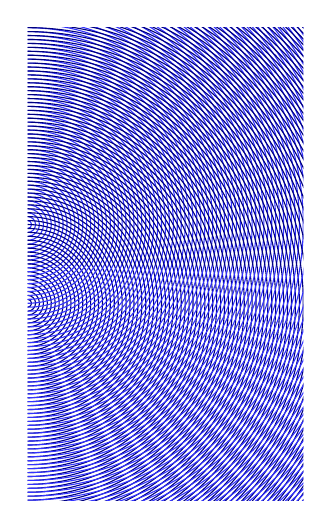
\begin{tikzpicture}%[scale=.6]
  \clip (0,-3)rectangle(3.5,3);
  \foreach \x in {0.05,0.1,...,5}
  {
    \draw[blue!80](0,0.5-\x)arc(-90:90:\x);
    \draw[blue!50!black](0,-0.5-\x)arc(-90:90:\x);
  }
\end{tikzpicture}
\end{document}